\documentclass[12pt]{article}
%\usepackage[document]{ragged2e}
\usepackage{array, amssymb, amsthm, linguex, enumerate, amsmath, physics, enumitem, xcolor, graphicx, xparse}
\let\fg\undefined %remove linguex/siunitx naming clash
\usepackage[english]{babel}
\usepackage[letterpaper,top=2cm,bottom=2cm,left=3cm,right=3cm,marginparwidth=1.75cm]{geometry}
\usepackage[colorlinks=true, allcolors=blue]{hyperref}
\usepackage[group-separator={,}]{siunitx} %\num{12345} -> "12,345"
\usepackage{fancyhdr}
\usepackage{notomath}
\usepackage[T1]{fontenc}
\usepackage{multicol}
\usepackage{mathtools}

%Number sets
\newcommand{\R}{\mathbb{R}}
\newcommand{\C}{\mathbb{C}}
\newcommand{\N}{\mathbb{N}}
\newcommand{\F}{\mathbb{F}}
\renewcommand{\Re}{\operatorname{Re}}
\renewcommand{\Im}{\operatorname{Im}}
\renewcommand{\L}[1]{\mathcal{L}\left({#1}\right)} %Linear Map

\newcommand{\pmp}{\,\pm\,} %add small extra space to \pm

\NewDocumentCommand{\ceil}{ s m }{% ceiling brackets
    \IfBooleanTF{#1}%
    {\lceil #2 \rceil}% starred: no-autosizing
    {\left\lceil #2 \right\rceil}% unstarred: autosizing
}

\NewDocumentCommand{\ceiling}{ s m }{% ceiling brackets
    \IfBooleanTF{#1}%
    {\lceil #2 \rceil}% starred: no-autosizing
    {\left\lceil #2 \right\rceil}% unstarred: autosizing
}

\NewDocumentCommand{\floor}{ s m }{% floor brackets
    \IfBooleanTF{#1}%
    {\lfloor #2 \rfloor}% starred: no-autosizing
    {\left\lfloor #2 \right\rfloor}% unstarred: autosizing
}

\NewDocumentCommand{\pars}{ s m }{% parenthesis
    \IfBooleanTF{#1}%
    {( #2 ) }% starred: no-autosizing
    {\left( #2 \right) }% unstarred: autosizing
}

\NewDocumentCommand{\inner}{ s m }{% inner product
    \IfBooleanTF{#1}%
    {\langle #2 \rangle}% starred: no-autosizing
    {\left\langle #2 \right\rangle}% unstarred: autosizing
}

\NewDocumentCommand{\innerconj}{ s m }{% inner product
    \IfBooleanTF{#1}%
    {\overline{\langle #2 \rangle}}% starred: no-autosizing
    {\overline{\left\langle #2 \right\rangle}}% unstarred: autosizing
}

\NewDocumentCommand{\brac}{ s m }{% brackets
    \IfBooleanTF{#1}%
    {[#2] }% starred: no-autosizing
    {\left[ #2 \right] }% unstarred: autosizing
}

%default latex bracket size naming
\newcommand{\biggbrac}[1]{\bigg[ {#1} \bigg] }
\newcommand{\bigbrac}[1]{\big[ {#1} \big] }
\newcommand{\Bigbrac}[1]{\Big[ {#1} \Big] }


\RenewDocumentCommand{\over}{ s m }{% fraction 1/arg
    \IfBooleanTF{#1}%
    {\dfrac{1}{#2}}% starred: dfrac
    {\frac{1}{#2}}% unstarred: normal frac
}

\NewDocumentCommand{\pover}{ s m }{% parenthesis around fraction (1/arg)
    \IfBooleanTF{#1}%
    {\left(\dfrac{1}{#2}\right)}% starred: dfrac
    {\left(\frac{1}{#2}\right)}% unstarred: normal frac
}

\NewDocumentCommand{\pfrac}{ s m m}{% parenthesis around fraction (arg1/arg2)
    \IfBooleanTF{#1}%
    {\left( \dfrac{{#2}}{{#3}} \right)}% starred: dfrac
    {\left( \frac{{#2}}{{#3}} \right)}% unstarred: normal frac
}


\newcommand{\Xbar}{\bar{X}}
\newcommand{\Ybar}{\bar{Y}}
\newcommand{\xbar}{\bar{x}}
\newcommand{\ybar}{\bar{y}}


\newcommand{\limn}{\lim_{n\to\infty}}
\newcommand{\limx}{\lim_{x\to\infty}}

\newcommand{\gammaDist}[2]{\operatorname{Gamma} \left( {#1},{#2} \right)} %gamma distribution
\NewDocumentCommand{\normalDist}{s g g}{ %normal distibution
    \IfBooleanTF{#1} { % starred, no autosizing parenthesis
      \IfNoValueTF{#2}{
          N (\mu,\, \sigma^2 ) %\normalDist* "default" normal distribution N(\mu, \sigma^2)
        } {
            \IfNoValueTF{#3}{N (#2)}{} %\normalDist{arg} --> N(arg)
        }
      \IfNoValueTF{#3}{}{N ( #2, #3 )}  %\normalDist*{arg1}{arg2} --> N(arg1,arg2)
    }  % else (unstarred) autosize parenthesis
    {
        \IfNoValueTF{#2}{
            N \left(\mu,\, \sigma^2 \right) %\normalDist "default" normal distribution N(\mu, \sigma^2)
        } {
            \IfNoValueTF{#3}{N \left(#2\right)}{} %\normalDist{arg} --> N(arg)
        }
        \IfNoValueTF{#3}{}{N \left( #2, #3 \right)} %\normalDist{arg1}{arg2} --> N(arg1,arg2)
    }
}



%colors
\definecolor{ggreen}{RGB}{0, 127, 0}
\definecolor{dgray}{RGB}{63,63,63}
\definecolor{neonorange}{RGB}{255,47,0}
\definecolor{mygray}{rgb}{0.5,0.5,0.5}
\definecolor{eblue}{RGB}{0,74,127}
\newcommand{\red}[1]{\color{red}{#1}\color{black}}
\newcommand{\green}[1]{\color{ggreen}{#1}\color{black}}
\newcommand{\blue}[1]{\color{blue}{#1}\color{black}}
\newcommand{\setRed}{\color{red}}
\newcommand{\setBlack}{\color{black}}
\newcommand{\setBlue}{\color{blue}}
\newcommand{\setGreen}{\color{ggreen}}



\newcommand{\thru}[1]{{#1}_1, \dots, {#1}_n}
\newcommand{\sumThru}[1]{{#1}_1 + \cdots + {#1}_n}
\newcommand{\yn}{Y_1, \dots, Y_n} % Y_1, ..., Y_n
\newcommand{\xn}{X_1, \dots, X_n} % Y_1, ..., Y_n

%hats and tildes
\newcommand{\that}{\widehat{\theta}} % theta hat
\newcommand{\phat}{\widehat{p}} % p hat
\newcommand{\qhat}{\widehat{q}} % p hat
\newcommand{\psihat}{\widehat{\psi}} % psi hat
\newcommand{\Psihat}{\widehat{\Psi}} % Psi hat
\newcommand{\ptilde}{\widetilde{p}} % psi tilde
\newcommand{\Psitil}{\widetilde{\Psi}} % Psi tilde
\newcommand{\betah}{\widehat{\beta}} % beta hat

%2x2 matrix shortcuts
\newcommand{\detx}[4]{\begin{vmatrix}{#1} & {#2}\\{#3}&{#4}\end{vmatrix}} % 2x2 determinant
\newcommand{\dety}[9]{\begin{vmatrix}{#1} & {#2} & {#3} \\{#4}&{#5}&{#6}\\ {#7} & {#8} & {#9}\end{vmatrix}} % 3x3 determinant
\newcommand{\bmaty}[9]{\begin{bmatrix}{#1} & {#2} & {#3} \\{#4}&{#5}&{#6}\\ {#7} & {#8} & {#9}\end{bmatrix}} % 3x3 matrix
\newcommand{\bmat}[4]{\begin{bmatrix}{#1} & {#2}\\{#3}&{#4}\end{bmatrix}} % 2x2 matrix brackets
\renewcommand{\pmat}[4]{\begin{pmatrix}{#1} & {#2}\\{#3}&{#4}\end{pmatrix}} % 2x2 matrix parenthesis

%remove any enumerate/itemize indent temporarily
\makeatletter   %% <- make @ usable in macro names
\newcommand*\notab[1]{%
  \begingroup   %% <- limit scope of the following changes
    \par        %% <- start a new paragraph
    \@totalleftmargin=0pt \linewidth=\columnwidth
    %% ^^ let other commands know that the margins have been reset
    \parshape 0
    %% ^^ reset the margins
    #1\par      %% <- insert #1 and end this paragraph
  \endgroup
}
\makeatother    %% <- revert @


\newcommand{\dimrange}[1]{\operatorname{dim}\operatorname{range}{#1}} % dimrange
\newcommand{\dimnull}[1]{\operatorname{dim}\operatorname{null}{#1}} % dimnull
\newcommand{\range}[1]{\operatorname{range}{#1}} %range
\newcommand{\nullspace}{\operatorname{null}} %null

% polynomial notation
\NewDocumentCommand{\poly}{ s g g }{%
    \IfBooleanTF{#1} {
        \IfNoValueTF{#2} {
            \mathcal{P}(\mathbb{R})
        } {
            \mathcal{P}_{#2}(\mathbb{R})
        }
    } {
        \IfNoValueTF{#3} {
            {\mathcal{P}(#2)}
        } { %else
            {\mathcal{P}_{#2}(#3)}
        }
    }
}

\NewDocumentCommand{\bias}{ s m }{% bias(arg)
    \IfBooleanTF{#1}%
    {\operatorname{bias}(#2)}% starred: no autosizing
    {\operatorname{bias}\left(#2\right)}% unstarred: autosizing
}

\NewDocumentCommand{\MSE}{ s m }{% MSE(arg)
    \IfBooleanTF{#1}%
    {\operatorname{MSE}(#2)}% starred: no autosizing
    {\operatorname{MSE}\left(#2\right)}% unstarred: autosizing
}

\NewDocumentCommand{\Var}{ s m }{% variance with parenthesis V(arg)
    \IfBooleanTF{#1}%
    {\operatorname{Var}(#2)}% starred: no autosizing
    {\operatorname{Var}\left(#2\right)}% unstarred: autosizing
}

\NewDocumentCommand{\Varb}{ s m }{% variance with brackets V[arg]
    \IfBooleanTF{#1}%
    {\operatorname{Var}[\,#2\,]}% starred: no autosizing
    {\operatorname{Var}\left[\,#2\,\right]}% unstarred: has autosizing
}

\NewDocumentCommand{\Vb}{ s m }{% another renaming of variance with brackets V[arg]
    \IfBooleanTF{#1}%
    {\operatorname{Var}[\,#2\,]}% starred: no autosizing
    {\operatorname{Var}\left[\,#2\,\right]}% unstarred: has autosizing
}

\NewDocumentCommand{\E}{ s m }{% expectation with parenthesis E(arg)
    \IfBooleanTF{#1}%
    {\operatorname{E}(#2)}% starred: no autosizing
    {\operatorname{E}\left(#2\right)}% unstarred: has autosizing
}

\NewDocumentCommand{\Eb}{ s m }{% expectation with brackets E[arg]
    \IfBooleanTF{#1}%
    {\operatorname{E}[#2]}% starred: no autosizing
    {\operatorname{E}\left[#2\right]}% unstarred: has autosizing
}

\RenewDocumentCommand{\P}{ s m }{% probability with parenthesis Pr(arg)
    \IfBooleanTF{#1}%
    {\Pr (#2) }% starred: no autosizing
    {\Pr \left( #2 \right) }% unstarred: has autosizing
}

\NewDocumentCommand{\prob}{ s m }{% probability with parenthesis Pr(arg)
    \IfBooleanTF{#1}%
    {\Pr (#2) }% starred: no autosizing
    {\Pr \left( #2 \right) }% unstarred: has autosizing
}

\NewDocumentCommand{\eff}{ s m }{% efficiency with parenthesis eff(arg)
    \IfBooleanTF{#1}%
    {\operatorname{eff}(#2)}% starred: no autosizing
    {\operatorname{eff}\left(#2\right)}% unstarred: has autosizing
}

%vertical vector of up to 8 elements
\NewDocumentCommand\vvec{s m g g g g g g g}{%
    \IfBooleanTF{#1} {
        \begin{bmatrix}% if starred use brackets
            \IfNoValueTF{#2}{}{#2}
            \IfNoValueTF{#3}{}{\\#3}
            \IfNoValueTF{#4}{}{\\#4}
            \IfNoValueTF{#5}{}{\\#5}
            \IfNoValueTF{#6}{}{\\#6}
            \IfNoValueTF{#7}{}{\\#7}
            \IfNoValueTF{#8}{}{\\#8}
        \end{bmatrix}
    }  % else (unstarred) use parethesis
    {
        \begin{pmatrix}%
            \IfNoValueTF{#2}{}{#2}
            \IfNoValueTF{#3}{}{\\#3}
            \IfNoValueTF{#4}{}{\\#4}
            \IfNoValueTF{#5}{}{\\#5}
            \IfNoValueTF{#6}{}{\\#6}
            \IfNoValueTF{#7}{}{\\#7}
            \IfNoValueTF{#8}{}{\\#8}
        \end{pmatrix}
    }
}
\def\Cov{\operatorname{Cov}} %Covariance
\def\df{\text{df}} %degrees of freedom

\NewDocumentCommand{\example}{ s g }{% Example header
    \IfBooleanTF{#1}%
    {\vspace{0.1in}}% starred: 0.1in
    {\vspace{0.2in}}% unstarred: 0.2in
    \IfNoValueTF{#2} {\noindent\textbf{\color{eblue} Example: }}{\noindent\textbf{\color{eblue} Example (#2): }}
}
\NewDocumentCommand{\disc}{ s }{% Discussion header
    \IfBooleanTF{#1}%
    {\vspace{0.1in}\noindent\textbf{Discussion: } }% starred: 0.1in
    {\vspace{0.2in}\noindent\textbf{Discussion: } }% unstarred: 0.2in
}
\NewDocumentCommand{\defn}{ s }{% Definition header
    \IfBooleanTF{#1}%
    {\vspace{0.1in}\noindent\textbf{\color{neonorange} Definition: } }% starred: 0.1in
    {\vspace{0.2in}\noindent\textbf{\color{neonorange} Definition: } }% unstarred: 0.2in
}
\NewDocumentCommand{\reason}{ s }{% Reason header
    \IfBooleanTF{#1}%
    {\vspace{0.1in}\noindent\textbf{Reason:} }% starred: 0.1in
    {\vspace{0.2in}\noindent\textbf{Reason:} }% unstarred: 0.2in
}
\NewDocumentCommand{\recall}{ s }{% Recall header
    \IfBooleanTF{#1}%
    {\vspace{0.1in}\noindent\textit{Recall:} }% starred: 0.1in
    {\vspace{0.2in}\noindent\textit{Recall:} }% unstarred: 0.2in
}
\NewDocumentCommand{\remark}{ s }{% Remark header
    \IfBooleanTF{#1}%
    {\vspace{0.1in}\noindent\textit{Remark:} }% starred: 0.1in
    {\vspace{0.2in}\noindent\textit{Remark:} }% unstarred: 0.2in
}

\NewDocumentCommand{\soln}{ s }{% Remark header
    \IfBooleanTF{#1}%
    {\vspace{0.1in}\noindent\textbf{Solution: } }% starred: 0.1in
    {\vspace{0.2in}\noindent\textbf{Solution: } }% unstarred: 0.2in
}

\newcommand{\proj}[2]{\operatorname{proj}_{{#1}}{#2}} %projection
\newcommand{\wideand}{\qquad \text{and} \qquad}

\newcommand{\bu}[1]{\textbf{\underline{{#1}}} } %bold underline
\newcommand{\boldit}[1]{\textbf{\textit{{#1}}} } %bold italix

% put actual quotation marks "around something"
\newcommand{\say}[1]{\textquotedblleft{#1}\textquotedblright}

% max{arg} and min{arg}
\renewcommand{\max}[1]{\operatorname{max}\left\{ #1 \right\}}
\renewcommand{\min}[1]{\operatorname{min}\left( #1 \right)}

\newcommand{\Span}[1]{\operatorname{span}\left\{ #1 \right\}}

%Create a new vspace line no indent
\newcommand{\nl}{\vspace{0.1in}\noindent}
\newcommand{\nnl}{\vspace{0.2in}\noindent}
\newcommand{\nnnl}{\vspace{0.3in}\noindent}
\textwidth=7.02in
\hoffset=-.425in

\setcounter{MaxMatrixCols}{20}
\begin{document}
\pagestyle{fancy}
\fancyhf{}
\fancyhead[RO]{Matthew Wilder}
\fancyhead[LO]{MTH 427 - Homework \#1}
\fancyfoot[CO]{Page \thepage}

\noindent MTH 427 - Spring 2023
\\Assignment \#1
\\Due: Monday, January 30th 2023 (11:59PM)

\section{Conceptual problems}
\begin{enumerate}
\item For any random variables $X$, $Y$ and any constants $a, b, c$ and $d$,
\\show that $\Cov(a+bX, c+dY) = bd \Cov(X,Y)$.

\begin{proof}
    \begin{align*}
        \Cov(a+bX, c+dY) &= \Eb{(a+bX)(c+dY)} - \Eb{a+bX}\Eb{c+dY}\\
        &= \Eb{ac+adY+bcX+bdXY} - \pars{\Eb{a}+\Eb{bX}}\pars{\Eb{c}+\Eb{dY} }\\
        &= ac + ad\Eb{Y} + bc\Eb{X} + bd\Eb{XY} - \pars{a + b\Eb{X}}\pars{c + d\Eb{Y}}\\
        &= ac + ad\Eb{Y} + bc\Eb{X} + bd\Eb{XY} - \pars{ac + ad\Eb{Y} + bc\Eb{X} + bd\Eb{X}\Eb{Y}}\\
        &= bd\Eb{XY} - bd\Eb{X}\Eb{Y} \tag{\say{Lots of killing} - McAsey}\\
        &= bd\pars{\Eb{XY} - \Eb{X}\Eb{Y}}\\
        &= bd \Cov(X,Y)
    \end{align*}
\end{proof}
\item Is the plant density of a species related to the altitude at which data are collected? Let $Y$ denote the species density and $X$ denote the altitude. A fit of a simple linear regression model using 14 observations yielded $\yhat = 21.6 - 7.79x$ and $r^2 = 0.61$.
\begin{enumerate}
\item What is the value of the correlation coefficient $r$?

\soln* $r^2 = 0.61 \iff r = \pm 0.781$, but because $\bat_1 < 0$ then $r = -0.781$.
\item If $\that_1$ and $\that_2$ are independent, how should $\alpha$ be chosen in order to minimize the variance of $\that_3$?

\soln* First derive the general form of the variance of the estimator $\that_3$. That is, 
\begin{align*}
    \Varb*{\that_3} &= \Varb*{\alpha \that_1 + (1-\alpha)\that_2} \tag{substitute}\\
    &= \alpha^2 \Varb*{\that_1} + (1-\alpha)^2 \Varb*{\that_2} + 2\alpha(1-\alpha) \Cov(\that_1, \that_2) \tag{formula}\\
    &= \alpha^2 \Varb*{\that_1} + (1-\alpha)^2 \Varb*{\that_2} \tag{By independence hypothesis}\\
    &= \alpha^2 {\sigma_1}^2 + (1-\alpha)^2 {\sigma_2}^2 \tag{substitute}
\end{align*}
Using the first derivative test wrt $\alpha$, 
$\displaystyle \pdv{\alpha} \pars{\alpha^2 {\sigma_1}^2 + (1-\alpha)^2 {\sigma_2}^2} = 2\alpha({\sigma_1}^2 + {\sigma_2}^2) + 2{\sigma_2}^2$. Setting this equal to 0 and solving for $\alpha$ yields 
$\alpha = \dfrac{{\sigma_2}^2}{{\sigma_1}^2+{\sigma_2}^2}$.

\end{enumerate}

\item Refer to exercise 11.3. Fit the model suggested there by use of matrices. 

\soln*
\begin{center}
    \begin{tabular}{l|ccccc}
         y & 3 & 2 & 1 & 1 & 0.5\\
         \hline
         x & -2 & -1 & 0 & 1 & 2\\
    \end{tabular}
\end{center}

$$
X = \begin{bmatrix}
	1 & -2\\
	1 & -1\\
	1 & 0\\
	1 & 1\\
	1 & 2\\
\end{bmatrix}
, \quad X^T =
\begin{bmatrix}
	1 & 1 & 1 & 1 & 1\\
	-2 & -1 & 0 & 1 & 2\\
\end{bmatrix}
, \quad Y=
\begin{bmatrix}
	3\\
	2\\
	1\\
	1\\
	0.5\\
\end{bmatrix}
$$
$$
X^TX = \begin{bmatrix}
	5 & 0\\
	0 & 10\\
\end{bmatrix}, \qquad (X^TX)^{-1} = \begin{bmatrix}
	\frac15 & 0\\
	0 & \frac{1}{10}\\
\end{bmatrix}
$$
$$
X^TY = \begin{bmatrix}
	7.5\\
	-6\\
\end{bmatrix}
$$
$$
\bat = (X^TX)^{-1}\cdot X^TY = \begin{bmatrix}
	\frac15 & 0\\
	0 & \frac{1}{10}\\
\end{bmatrix}
\begin{bmatrix}
	7.5\\
	-6\\
\end{bmatrix} = \begin{bmatrix}
	1.5\\
	-0.6\\
\end{bmatrix}
$$
$$\therefore \yhat = -0.6x + 1.5$$
\end{enumerate}
\section{Applied problems - R}
\begin{enumerate}
    \item This exercise relates to the \say{Credit} dataset, which can be found as \say{Credit.csv} in Canvas.
\begin{enumerate}
    \item Use the appropriate function in R to produce a numerical summary of the quantitative variables in the
data.

\noindent 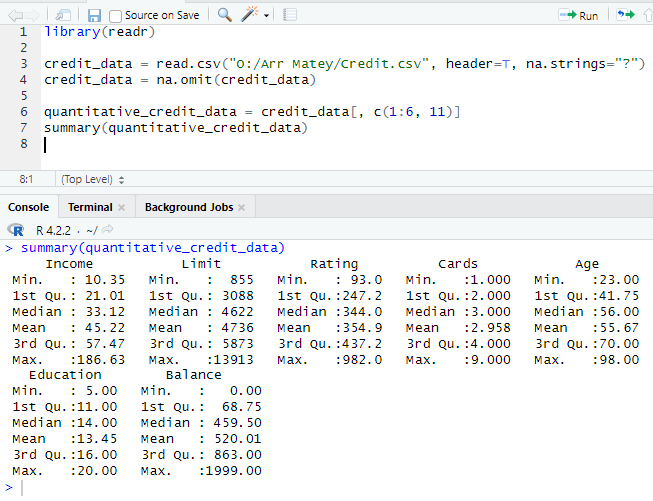
\includegraphics[width=6in]{r_1a.PNG}
    \item Display a scatter plot matrix between quantitative variables in the data set.

\noindent 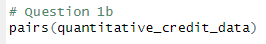
\includegraphics[width=2in]{r_1b-1.PNG}

\noindent 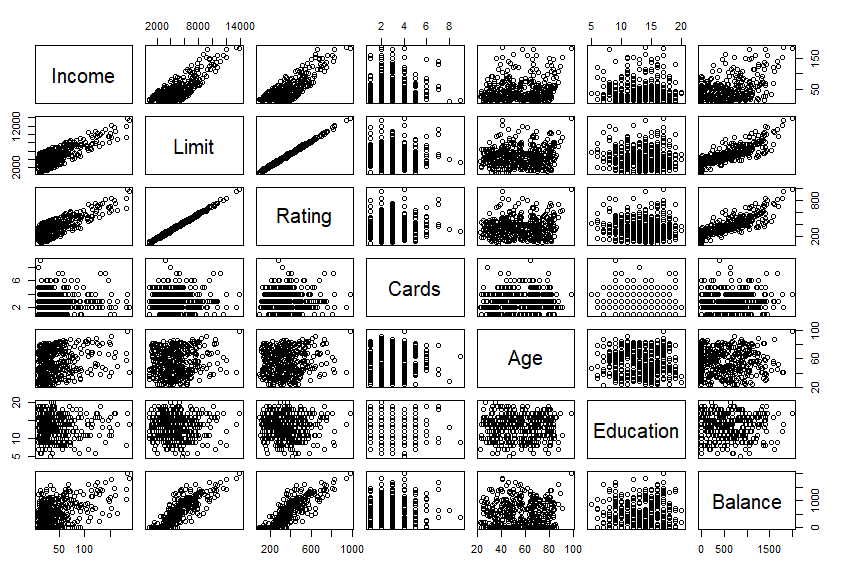
\includegraphics[width=6in]{r_1b-2.PNG}\newpage
    \item Display histograms of all quantitative variables in one graph except \say{cards} (side by side). You may
use different colors.

\noindent 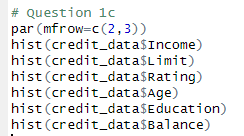
\includegraphics[width=2in]{r_1c-1.PNG}

\noindent 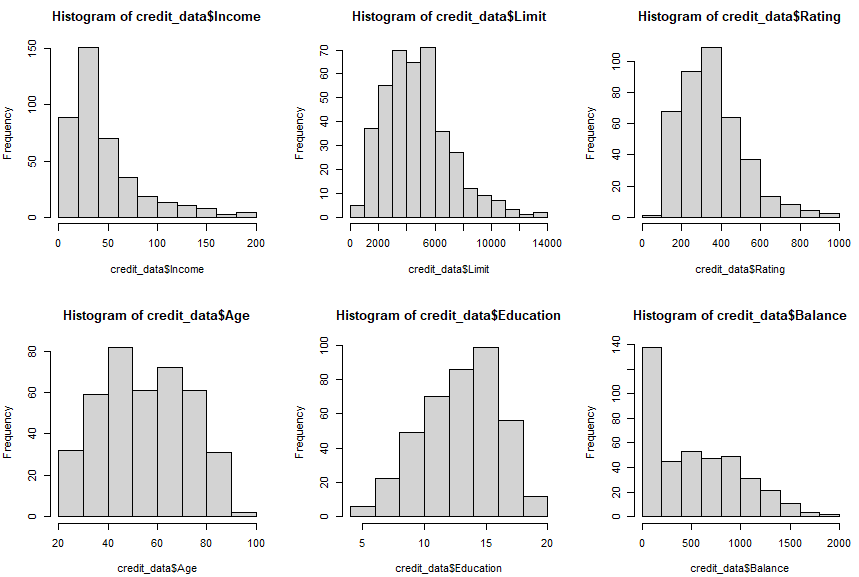
\includegraphics[width=6in]{r_1c-2.PNG}\newpage
    \item Display box-plots of all quantitative variables only in one graph except \say{cards} (side by side). Make
sure to label them.

\noindent 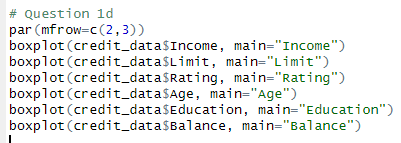
\includegraphics[width=3in]{r_1d-1.PNG}

\noindent 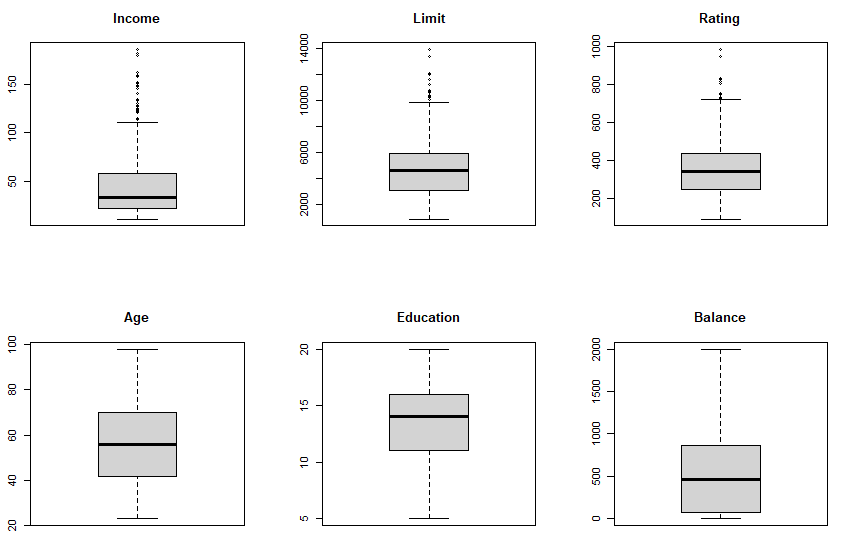
\includegraphics[width=6in]{r_1d-2.PNG}
\end{enumerate}\newpage
    \item This exercise relates to the \say{Hwk-data1} dataset, which can be found in Canvas.

\nl Operators of gasoline-fueled vehicles complain about the price of gasoline in gas stations. According to
the American Petroleum Institute, the federal gas tax per gallon is constant (18.4 cents as of January
13, 2005), but state and local taxes vary from 7.5 cents to 32.10 cents for $n = 18$ key metropolitan areas
around the country.

\nl \textit{Use R for part (a), (b), and (c)}

\begin{enumerate}
    \item Check whether the data are normally distributed by using the Shapiro test or by looking at the QQ
plot. (Make sure to display your results).

\noindent 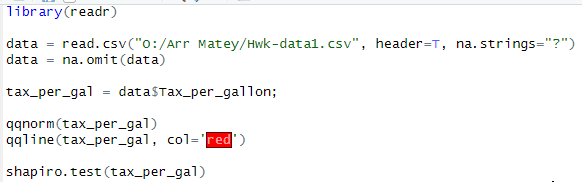
\includegraphics[width=5in]{r_2a-1.PNG}

\noindent 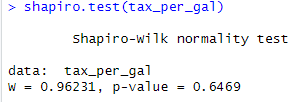
\includegraphics[width=3in]{r_2a-3.PNG}

\noindent Since $p = 0.6469 > \alpha$ (assuming $\alpha = 0.05$), the data are normally distributed.

\noindent 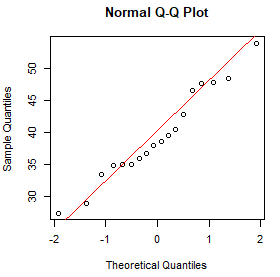
\includegraphics[width=3.5in]{r_2a-2.PNG}\newpage
    \item Use the appropriate R function to find a 90\% confidence interval for the average per gallon gas tax in
the U.S. (Make sure to display your code and the corresponding result.)

\noindent 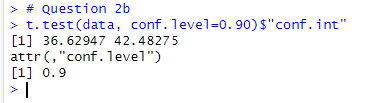
\includegraphics[width=3.5in]{r_2b.PNG}

\noindent The confidence interval $I := (36.62947, 42.48275)$.\vspace{0.3in}
    \item Is there sufficient evidence to claim that the average gas tax is less that 45.2 cents? (Make sure to
specify hypotheses and the p-value).

\soln* $H_0 := \mu = 45.2$ and $H_a := \mu < 45.2$.

\noindent 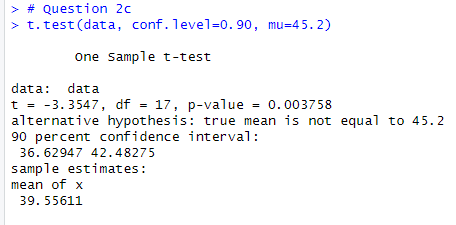
\includegraphics[width=3.5in]{r_2c.PNG}

\noindent Since $p =0.003758 \leq 0.1 = \alpha$, we reject the null hypothesis ($H_0$). Hence, there is sufficient evidence that the true mean of the gas tax is less than 45.2 cents.\vspace{0.3in}
    \item Compute (by hand) a 98\% confidence interval for the average per gallon gas tax in the U.S. Compare
the length of this interval and the one in part (b). (Hint: the sample standard deviation $s = 7.138$)

\soln* $\Xbar \approx 39.556$, $\df = 18-1 = 17$, and $\alpha = 0.02$. Then $t_{\alpha/2}(17) = t_{0.01}(17) = 2.567$.

\nl Then the CI is $39.556 \pm 2.567 \pfrac{7.138}{\sqrt{18}} \equiv (35.237, 43.875)$. The measure of this interval is $8.638$ cents, whereas in part (b) the measure was $5.85328$ cents. Higher confidence levels require more of the domain since $\lim_{\alpha \to 0^+} \equiv D$. 
\end{enumerate}
    \end{enumerate}


\end{document}
